\title{Solomonoff Library Specification and Technical Documentation}
\author{Aleksander Mendoza-Drosik}

\documentclass[12pt]{article}
\usepackage{tikz}
\usepackage[utf8]{inputenc}
\usepackage[T1]{fontenc}
\usepackage{lmodern}
\usepackage{amsfonts}
\usepackage{mathrsfs}
\usepackage{centernot}
\usepackage{listings}
\usepackage{mathtools}
\usepackage{xcolor}
\usepackage{url}
\usepackage{hyperref}
\usepackage{amsthm}
\usepackage{amsmath}
\usepackage{amssymb}
\usepackage{syntax}
\newtheorem{definition}{Definition}
\newtheorem{theorem}{Theorem}[section]
\newtheorem{corollary}{Corollary}[theorem]
\newtheorem{lemma}[theorem]{Lemma}
\renewcommand{\labelenumii}{\theenumii}
\renewcommand{\theenumii}{\theenumi.\arabic{enumii}.}
\DeclareMathSymbol{:}{\mathord}{operators}{"3A}

\begin{document}
\maketitle
\lstset{
	basicstyle=\ttfamily,
	mathescape
}


The theory behind implementation and design of Solomonoff has been studied and developed over the course of 2 years. The early versions and our initial ideas looked very different to the final results we've achieved. 

At the beginning it was meant to be a simple tools that focused only on deterministic Mealy automata. Such a model was very limited and it quickly became apparent that certain extensions would need to be made. In the end we implemented a compiler that supports nondeterministic functional weighted symbolic transducers. 

\section{Mealy automata and transducers}

The standard definition of automaton found in introductory courses states that finite state automaton is  a tuple $(Q,I,\delta,F,\Sigma)$ where $Q$ is the set of states, $I \subset Q$ are the initial states,  $F \subset Q$ are the final (or accepting) states, $\delta:Q\times \Sigma \rightarrow Q$ is the transition function and $\Sigma$ is some alphabet. 

A Mealy machine extends the above definition with output  $(Q,I,\delta,F,\Sigma,\Gamma)$ where $\Gamma$ is some output alphabet and transition function has the form of $\delta:Q\times \Sigma \rightarrow Q \times \Gamma$. 

Such a model is frequently used in the field of formal methods. Many complex state-based systems can be modelled and simplified using Mealy machines. As an example consider a black-box computer program whose logs can be observed. The current snapshot of the program's memory determines its state. Depending on subsequent user input, we might observe different log traces. There are many existing machine learning and inference algorithms that can build an equivalent model of Mealy machine only by interacting with such a black-box system and reading its logs. 

It can be proved that the expressive power of deterministic automata with output is strictly less than that of their nondeterministic counterparts. It is known as the prefix-preserving  property. If a deterministic automaton reads input string $\sigma_1\sigma_2\sigma_1$ and prints $\gamma_1\gamma_1\gamma_2$, then at the next step it is only allowed to append one more symbol to the previously generated output. For instance we could not suddenly change the output to $\gamma_2\gamma_2\gamma_2\gamma_1$ after reading one more input symbol $\sigma_1\sigma_2\sigma_1\sigma_2$. The prefix $\gamma_1\gamma_1\gamma_2$ must be preserved. 

The problems that we wanted to tackle with Solomonoff revolved around building sequence-to-sequence models. For instance we might want to translate from numbers written as English words into digits. A sentence like "one apple" should become "1 apple". The prefix preserving property would be too limiting because it often happens that the suffix of string has decisive impact on the translation. The phrase "once again"
also starts with prefix "one" but it should not be translated as "1ce again"!

We intended to find the right balance between expressive power of nondeterministic machines and strong formal guarantees of Mealy automata. To achieve this, we initially decided to use multitape automata. The idea was to write all possible continuations of given output and store each in a separate output tape. Then upon reaching the end of string, the state would decide which tape to use as output. 

Over the course of research and development we have discovered that the power of multitape Mealy machines was still too limiting for our purposes. In particular we could define congruence classes on pairs of strings similar to those in Myhill-Nerode theorem. Then it can be easily noticed that as long as the number of output tapes is finite, the number of congruence classes must be finite as well. A very simple counter-example would the language that for every string $a$, $aa$, $aaa$,... respectively prints output $c$, $bc$, $bbc$,...and so on. It could not be expressed using only a finite number of output tapes, because there are infinitely many ways to continue the output and none of them is a prefix of the other.  



Yet another limitation of Mealy machines is that their $\delta$ function enforces outputs of the exact same length as inputs. In the field of natural language processing such an assumption is too strict. For instance, we might want to 
build a machine that translates sentences from one language to another. A word "fish" in English might have 4 letters but Spanish "pescado" is much longer. Our first idea was to use sequential transducers instead of the plain Mealy automata. Their definition allows the transition function to print output strings of arbitrary length $\delta:Q\times \Sigma \rightarrow Q^*$. 


The nondeterministic transducers  don't suffer from any of the above problems. Their expressive power exactly corresponds to that of regular transductions. It's a very strong and expressive class. The only way to obtain a stronger model would be by introducing context-free grammars and pushdown automata. The reason why we were hesitant to use this approach was because of the possible ambiguity of output. Nondeterministic transducers may contain epsilon transitions, which could lead to infinite number of outputs for any given input. Without epsilons, the number of outputs is finite but it's still possible to return more than one ambiguous output.

The model of automata that was finally implemented in Solomonoff, are the functional nondeterministic transducers. Functionality of transducer means that for any input, there may be at most one output. For instance the transducer below is not functional, because for input string $abb$ it prints both outputs $xyx$ and $yxx$. 
\begin{center}
	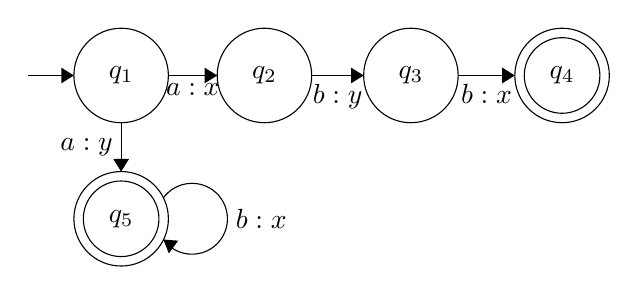
\begin{tikzpicture}[scale=0.2]
		\tikzstyle{every node}+=[inner sep=0pt]
		\draw [black] (40.2,-18) circle (3);
		\draw (40.2,-18) node {$q_4$};
		\draw [black] (40.2,-18) circle (2.4);
		\draw [black] (12.2,-18) circle (3);
		\draw (12.2,-18) node {$q_1$};
		\draw [black] (21.3,-18) circle (3);
		\draw (21.3,-18) node {$q_2$};
		\draw [black] (12.2,-27.1) circle (3);
		\draw (12.2,-27.1) node {$q_5$};
		\draw [black] (12.2,-27.1) circle (2.4);
		\draw [black] (30.6,-18) circle (3);
		\draw (30.6,-18) node {$q_3$};
		\draw [black] (15.2,-18) -- (18.3,-18);
		\fill [black] (18.3,-18) -- (17.5,-17.5) -- (17.5,-18.5);
		\draw (16.75,-18.5) node [below] {$a:x$};
		\draw [black] (6.3,-18) -- (9.2,-18);
		\fill [black] (9.2,-18) -- (8.4,-17.5) -- (8.4,-18.5);
		\draw [black] (24.3,-18) -- (27.6,-18);
		\fill [black] (27.6,-18) -- (26.8,-17.5) -- (26.8,-18.5);
		\draw (25.95,-18.5) node [below] {$b:y$};
		\draw [black] (33.6,-18) -- (37.2,-18);
		\fill [black] (37.2,-18) -- (36.4,-17.5) -- (36.4,-18.5);
		\draw (35.4,-18.5) node [below] {$b:x$};
		\draw [black] (12.2,-21) -- (12.2,-24.1);
		\fill [black] (12.2,-24.1) -- (12.7,-23.3) -- (11.7,-23.3);
		\draw (11.7,-22.55) node [left] {$a:y$};
		\draw [black] (14.88,-25.777) arc (144:-144:2.25);
		\draw (19.45,-27.1) node [right] {$b:x$};
		\fill [black] (14.88,-28.42) -- (15.23,-29.3) -- (15.82,-28.49);
	\end{tikzpicture}
\end{center}
This should not be confused with unambiguous automata. For example the transducer below is functional but ambiguous. The input $abb$ prints only a single output $yxx$, albeit there are two ambiguous accepting path that produce it.
\begin{center}
	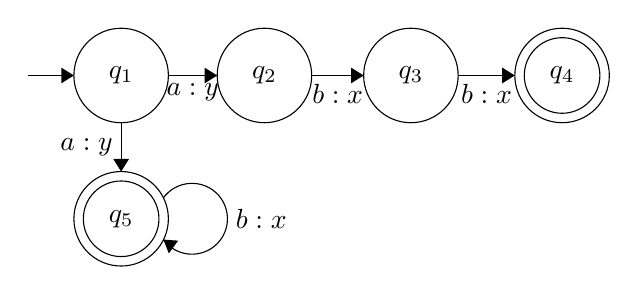
\begin{tikzpicture}[scale=0.2]
		\tikzstyle{every node}+=[inner sep=0pt]
		\draw [black] (40.2,-18) circle (3);
		\draw (40.2,-18) node {$q_4$};
		\draw [black] (40.2,-18) circle (2.4);
		\draw [black] (12.2,-18) circle (3);
		\draw (12.2,-18) node {$q_1$};
		\draw [black] (21.3,-18) circle (3);
		\draw (21.3,-18) node {$q_2$};
		\draw [black] (12.2,-27.1) circle (3);
		\draw (12.2,-27.1) node {$q_5$};
		\draw [black] (12.2,-27.1) circle (2.4);
		\draw [black] (30.6,-18) circle (3);
		\draw (30.6,-18) node {$q_3$};
		\draw [black] (15.2,-18) -- (18.3,-18);
		\fill [black] (18.3,-18) -- (17.5,-17.5) -- (17.5,-18.5);
		\draw (16.75,-18.5) node [below] {$a:y$};
		\draw [black] (6.3,-18) -- (9.2,-18);
		\fill [black] (9.2,-18) -- (8.4,-17.5) -- (8.4,-18.5);
		\draw [black] (24.3,-18) -- (27.6,-18);
		\fill [black] (27.6,-18) -- (26.8,-17.5) -- (26.8,-18.5);
		\draw (25.95,-18.5) node [below] {$b:x$};
		\draw [black] (33.6,-18) -- (37.2,-18);
		\fill [black] (37.2,-18) -- (36.4,-17.5) -- (36.4,-18.5);
		\draw (35.4,-18.5) node [below] {$b:x$};
		\draw [black] (12.2,-21) -- (12.2,-24.1);
		\fill [black] (12.2,-24.1) -- (12.7,-23.3) -- (11.7,-23.3);
		\draw (11.7,-22.55) node [left] {$a:y$};
		\draw [black] (14.88,-25.777) arc (144:-144:2.25);
		\draw (19.45,-27.1) node [right] {$b:x$};
		\fill [black] (14.88,-28.42) -- (15.23,-29.3) -- (15.82,-28.49);
	\end{tikzpicture}
\end{center}
Functional nondeterministic transducers proved to provide the perfect balance of power with many strong formal guarantees. While epsilon transitions strictly increase power of transducers, when restricted only to functional automata, the erasure of epsilons becomes possible. Using advance-and-delay algorithm one can test functionality of any automaton in quadratic time. There exists a special version of powerset construction that can take any functional transducers and produce an equivalent unambiguous automaton. One can take advantage of unambiguity to build an inference algorithm for learning functional automata from sample data.  The automata are closed under union, concatenation, Kleene closure and composition. Unlike non-functional transducers, they are not closed under inversion but we developed a special algebra that uniquely defines an invertible  bijective transduction for any automaton. Glushkov's construction can be augmented to produce functional transducers.  Lexicographic semiring of weights can be used to make functional automata more compact.  


Once we decided to use the power of functional transducers, the next problem we had to solve was their optimisation. One of the most important operations in natural language processing is the context-dependent rewrite. The standard way of implementing it is by building a large transducer that handles all possible cases.
In Solomonoff we've developed our own approach that produces much smaller automata. It is done with lexicographic weights.

Another important optimisation is the state minimisation. Many existing libraries implement separate functions for all regular operations and additional one for minimisation. A regular expression like $A(B+C)*$ would be then translated to a series of function calls like 
\[
minimise(concatenate(A,kleene\_closure(union(B,C)))) 
\]
This was out initial idea too but later we stumbled upon a better approach. In Solomonoff we don't have separate implementation for those operations. Instead everything is integrated in form of one monolithic procedure that implements Glushkov's construction. For example, in order to compile the expression
\[
aa(b+ca)*+c
\] we first convert every symbol into a state and obtain the following intermediate "regular expression"  
\[
q_1q_2(q_3+q_4 q_5)*+q_6
\]
Then we add one more state at the beginning that will serve as initial
\[
q_0(q_1q_2(q_3+q_4 q_5)*+q_6)
\]
Next we analyse it and determine, which state can be reached from any other. After "reading" $q_1$ we can "read" $q_2$. After $q_2$ we can either read $q_3$ or $q_4$. After $q_3$ we can read either $q_3$ again or go to $q_4$. Analogically for the remaining states. We also check, which states can appear at the end of the regular expression. In this example $q_2$, $q_3$, $q_5$ and $q_6$ are the final states because reading may end after reaching them. By putting all the above information together, we are able to produce the following automaton.

\begin{center}
	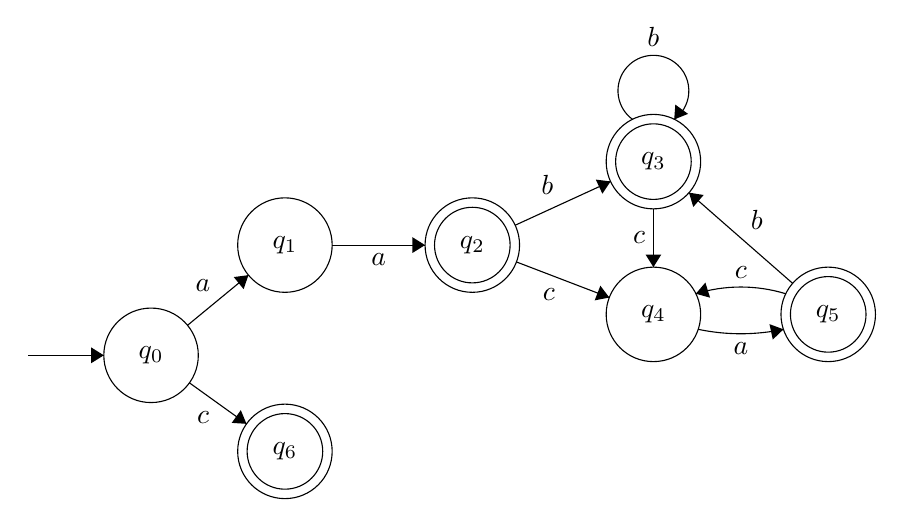
\begin{tikzpicture}[scale=0.2]
		\tikzstyle{every node}+=[inner sep=0pt]
		\draw [black] (21.6,-19.8) circle (3);
		\draw (21.6,-19.8) node {$q_1$};
		\draw [black] (13.1,-26.8) circle (3);
		\draw (13.1,-26.8) node {$q_0$};
		\draw [black] (33.5,-19.8) circle (3);
		\draw (33.5,-19.8) node {$q_2$};
		\draw [black] (33.5,-19.8) circle (2.4);
		\draw [black] (45,-14.5) circle (3);
		\draw (45,-14.5) node {$q_3$};
		\draw [black] (45,-14.5) circle (2.4);
		\draw [black] (45,-24.2) circle (3);
		\draw (45,-24.2) node {$q_4$};
		\draw [black] (56.1,-24.2) circle (3);
		\draw (56.1,-24.2) node {$q_5$};
		\draw [black] (56.1,-24.2) circle (2.4);
		\draw [black] (21.6,-32.9) circle (3);
		\draw (21.6,-32.9) node {$q_6$};
		\draw [black] (21.6,-32.9) circle (2.4);
		\draw [black] (5.3,-26.8) -- (10.1,-26.8);
		\fill [black] (10.1,-26.8) -- (9.3,-26.3) -- (9.3,-27.3);
		\draw [black] (15.42,-24.89) -- (19.28,-21.71);
		\fill [black] (19.28,-21.71) -- (18.35,-21.83) -- (18.98,-22.6);
		\draw (16.4,-22.81) node [above] {$a$};
		\draw [black] (24.6,-19.8) -- (30.5,-19.8);
		\fill [black] (30.5,-19.8) -- (29.7,-19.3) -- (29.7,-20.3);
		\draw (27.55,-20.3) node [below] {$a$};
		\draw [black] (36.22,-18.54) -- (42.28,-15.76);
		\fill [black] (42.28,-15.76) -- (41.34,-15.64) -- (41.76,-16.54);
		\draw (38.27,-16.64) node [above] {$b$};
		\draw [black] (36.3,-20.87) -- (42.2,-23.13);
		\fill [black] (42.2,-23.13) -- (41.63,-22.38) -- (41.27,-23.31);
		\draw (38.36,-22.52) node [below] {$c$};
		\draw [black] (53.261,-25.148) arc (-78.08261:-101.91739:13.126);
		\fill [black] (53.26,-25.15) -- (52.37,-24.82) -- (52.58,-25.8);
		\draw (50.55,-25.93) node [below] {$a$};
		\draw [black] (47.687,-22.893) arc (107.10284:72.89716:9.734);
		\fill [black] (47.69,-22.89) -- (48.6,-23.14) -- (48.3,-22.18);
		\draw (50.55,-21.96) node [above] {$c$};
		\draw [black] (53.84,-22.23) -- (47.26,-16.47);
		\fill [black] (47.26,-16.47) -- (47.53,-17.38) -- (48.19,-16.62);
		\draw (51.56,-18.86) node [above] {$b$};
		\draw [black] (45,-17.5) -- (45,-21.2);
		\fill [black] (45,-21.2) -- (45.5,-20.4) -- (44.5,-20.4);
		\draw (44.5,-19.35) node [left] {$c$};
		\draw [black] (43.677,-11.82) arc (234:-54:2.25);
		\draw (45,-7.25) node [above] {$b$};
		\fill [black] (46.32,-11.82) -- (47.2,-11.47) -- (46.39,-10.88);
		\draw [black] (15.54,-28.55) -- (19.16,-31.15);
		\fill [black] (19.16,-31.15) -- (18.8,-30.28) -- (18.22,-31.09);
		\draw (16.4,-30.35) node [below] {$c$};
	\end{tikzpicture}
\end{center}
This way the produced automata are very small even without the need for minimisation. If the regular expression consists of $n$ input symbols, then the resulting transducers has $n+1$ states. Because there is one-to-one correspondence between regular expression symbols and automata states, we are able to retain plenty of useful meta information. In particular each state can tell us exactly, which source file it comes from and the precise position in that file.  
This way, whenever compilation fails, user can see meaningful error messages.


The standard minimisation procedure used by most libraries works by finding the unique smallest deterministic automaton. Nondeterministic automata do not admit unique smallest representative and might be even exponentially smaller than their equivalent minimal deterministic counterparts. Finding the smallest possible nondeterministic automaton is a hard problem. For this reason Solomonoff implements a heuristic pseudo-minimisation algorithm that attempts to compress nondeterministic transducers and does not attempt to determinise them. Glushkov's construction already produces very small automata, hence any attempt at minimising them by determinisation would result in larger automata than the initial ones. Solomonoff's minimisation is inspired by Brzozowski's algorithm and is based on the duality of reachable and unobservable states. In simple terms, if two states have the exact same  sets of incoming (or outgoing) transitions then they have no reachable (or observable) distinguishing sequence. For example in the fragment of automaton below, the states $q_5$ and $q_6$ are indistinguishable because they have the exact same incoming transitions. As a result, reaching one state always implies also reaching the other.

\begin{center}
	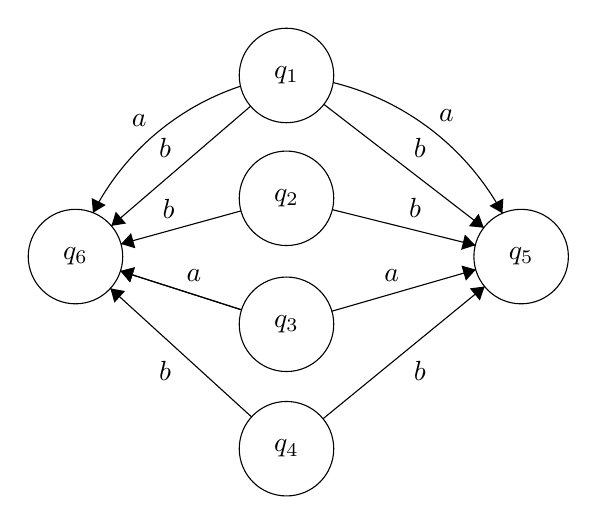
\begin{tikzpicture}[scale=0.2]
		\tikzstyle{every node}+=[inner sep=0pt]
		\draw [black] (26,-20.5) circle (3);
		\draw (26,-20.5) node {$q_2$};
		\draw [black] (26,-28.5) circle (3);
		\draw (26,-28.5) node {$q_3$};
		\draw [black] (26,-12.7) circle (3);
		\draw (26,-12.7) node {$q_1$};
		\draw [black] (26,-36.4) circle (3);
		\draw (26,-36.4) node {$q_4$};
		\draw [black] (40.9,-24.2) circle (3);
		\draw (40.9,-24.2) node {$q_5$};
		\draw [black] (12.6,-24.2) circle (3);
		\draw (12.6,-24.2) node {$q_6$};
		\draw [black] (28.962,-13.151) arc (76.21947:28.45774:16.774);
		\fill [black] (39.71,-21.45) -- (39.77,-20.51) -- (38.89,-20.98);
		\draw (36.16,-15.67) node [above] {$a$};
		\draw [black] (28.91,-21.22) -- (37.99,-23.48);
		\fill [black] (37.99,-23.48) -- (37.33,-22.8) -- (37.09,-23.77);
		\draw (34.17,-21.78) node [above] {$b$};
		\draw [black] (28.88,-27.67) -- (38.02,-25.03);
		\fill [black] (38.02,-25.03) -- (37.11,-24.77) -- (37.39,-25.73);
		\draw (32.68,-25.8) node [above] {$a$};
		\draw [black] (23.78,-34.38) -- (14.82,-26.22);
		\fill [black] (14.82,-26.22) -- (15.07,-27.13) -- (15.75,-26.39);
		\draw (18.29,-30.79) node [below] {$b$};
		\draw [black] (23.14,-27.58) -- (15.46,-25.12);
		\fill [black] (15.46,-25.12) -- (16.07,-25.84) -- (16.37,-24.88);
		\draw (20.12,-25.81) node [above] {$a$};
		\draw [black] (28.32,-34.5) -- (38.58,-26.1);
		\fill [black] (38.58,-26.1) -- (37.64,-26.22) -- (38.28,-26.99);
		\draw (34.46,-30.79) node [below] {$b$};
		\draw [black] (23.14,-27.58) -- (15.46,-25.12);
		\fill [black] (15.46,-25.12) -- (16.07,-25.84) -- (16.37,-24.88);
		\draw [black] (23.11,-21.3) -- (15.49,-23.4);
		\fill [black] (15.49,-23.4) -- (16.4,-23.67) -- (16.13,-22.71);
		\draw (18.51,-21.79) node [above] {$b$};
		\draw [black] (13.714,-21.419) arc (152.89319:108.37979:16.297);
		\fill [black] (13.71,-21.42) -- (14.52,-20.93) -- (13.63,-20.48);
		\draw (16.65,-15.99) node [above] {$a$};
		\draw [black] (23.72,-14.65) -- (14.88,-22.25);
		\fill [black] (14.88,-22.25) -- (15.81,-22.1) -- (15.16,-21.35);
		\draw (18.29,-17.96) node [above] {$b$};
		\draw [black] (28.37,-14.53) -- (38.53,-22.37);
		\fill [black] (38.53,-22.37) -- (38.2,-21.48) -- (37.59,-22.27);
		\draw (34.46,-17.95) node [above] {$b$};
	\end{tikzpicture}
\end{center}
Analogically in the example below the states also are indistinguishable but this time the outgoing transitions are the same. Hence the effects of reaching one state are equivalent to the other.

\begin{center}
	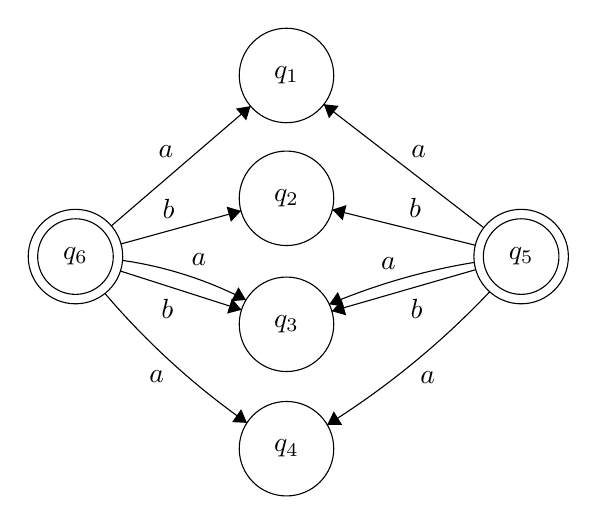
\begin{tikzpicture}[scale=0.2]
		\tikzstyle{every node}+=[inner sep=0pt]
		\draw [black] (26,-20.5) circle (3);
		\draw (26,-20.5) node {$q_2$};
		\draw [black] (26,-28.5) circle (3);
		\draw (26,-28.5) node {$q_3$};
		\draw [black] (26,-12.7) circle (3);
		\draw (26,-12.7) node {$q_1$};
		\draw [black] (26,-36.4) circle (3);
		\draw (26,-36.4) node {$q_4$};
		\draw [black] (40.9,-24.2) circle (3);
		\draw (40.9,-24.2) node {$q_5$};
		\draw [black] (40.9,-24.2) circle (2.4);
		\draw [black] (12.6,-24.2) circle (3);
		\draw (12.6,-24.2) node {$q_6$};
		\draw [black] (12.6,-24.2) circle (2.4);
		\draw [black] (14.88,-22.25) -- (23.72,-14.65);
		\fill [black] (23.72,-14.65) -- (22.79,-14.8) -- (23.44,-15.55);
		\draw (18.35,-17.96) node [above] {$a$};
		\draw [black] (15.49,-23.4) -- (23.11,-21.3);
		\fill [black] (23.11,-21.3) -- (22.2,-21.03) -- (22.47,-21.99);
		\draw (18.51,-21.79) node [above] {$b$};
		\draw [black] (15.588,-24.443) arc (81.8543:62.5633:24.571);
		\fill [black] (23.43,-26.96) -- (22.95,-26.15) -- (22.49,-27.03);
		\draw (20.44,-24.83) node [above] {$a$};
		\draw [black] (23.491,-34.756) arc (-125.02905:-139.6034:48.083);
		\fill [black] (23.49,-34.76) -- (23.12,-33.89) -- (22.55,-34.71);
		\draw (17.76,-31.42) node [below] {$a$};
		\draw [black] (38.53,-22.37) -- (28.37,-14.53);
		\fill [black] (28.37,-14.53) -- (28.7,-15.42) -- (29.31,-14.63);
		\draw (34.4,-17.95) node [above] {$a$};
		\draw [black] (37.99,-23.48) -- (28.91,-21.22);
		\fill [black] (28.91,-21.22) -- (29.57,-21.9) -- (29.81,-20.93);
		\draw (34.17,-21.78) node [above] {$b$};
		\draw [black] (28.716,-27.227) arc (112.97017:99.22512:40.045);
		\fill [black] (28.72,-27.23) -- (29.65,-27.38) -- (29.26,-26.45);
		\draw (32.47,-25.07) node [above] {$a$};
		\draw [black] (38.901,-26.436) arc (-43.42542:-57.9539:52.712);
		\fill [black] (28.59,-34.88) -- (29.53,-34.88) -- (29,-34.03);
		\draw (34.96,-31.48) node [below] {$a$};
		\draw [black] (15.46,-25.12) -- (23.14,-27.58);
		\fill [black] (23.14,-27.58) -- (22.53,-26.86) -- (22.23,-27.82);
		\draw (18.43,-26.89) node [below] {$b$};
		\draw [black] (38.02,-25.03) -- (28.88,-27.67);
		\fill [black] (28.88,-27.67) -- (29.79,-27.93) -- (29.51,-26.97);
		\draw (34.26,-26.9) node [below] {$b$};
	\end{tikzpicture}
\end{center}
The states $q_5$ and $q_6$ can be merged without affecting the language of automaton. Such a pseudo-minimisation procedure has been chosen, because it works especially well when combined with Glushkov's construction. The process of merging indistinguishable states is analogical to the process of isolating common parts of regular expression. For example the following
\[
ab+aab+ac(b+bb)
\]
could be shortened to 
\[
a(\epsilon+a+c(\epsilon+b))b
\]
by isolating the common prefix $a$ and suffix $b$. Extracting common prefixes exactly correspond to merging states with identical incoming transition, while common suffixes correspond to states with the same outgoing transitions. Sometimes there are cases that do not have any common prefix/suffix in the regular expression itself but still produce indistinguishable states in the automaton. For instance consider
\[
a+b+c+d+e
\]
which yields automaton

\begin{center}
	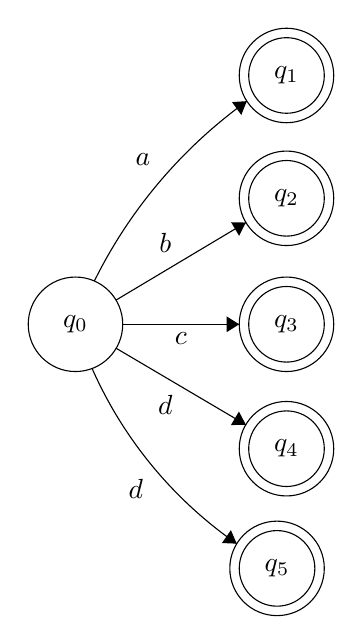
\begin{tikzpicture}[scale=0.2]
		\tikzstyle{every node}+=[inner sep=0pt]
		\draw [black] (26,-20.5) circle (3);
		\draw (26,-20.5) node {$q_2$};
		\draw [black] (26,-20.5) circle (2.4);
		\draw [black] (26,-28.5) circle (3);
		\draw (26,-28.5) node {$q_3$};
		\draw [black] (26,-28.5) circle (2.4);
		\draw [black] (26,-12.7) circle (3);
		\draw (26,-12.7) node {$q_1$};
		\draw [black] (26,-12.7) circle (2.4);
		\draw [black] (26,-36.4) circle (3);
		\draw (26,-36.4) node {$q_4$};
		\draw [black] (26,-36.4) circle (2.4);
		\draw [black] (12.6,-28.5) circle (3);
		\draw (12.6,-28.5) node {$q_0$};
		\draw [black] (25.4,-44) circle (3);
		\draw (25.4,-44) node {$q_5$};
		\draw [black] (25.4,-44) circle (2.4);
		\draw [black] (13.799,-25.751) arc (153.65447:125.74289:31.042);
		\fill [black] (23.48,-14.33) -- (22.54,-14.39) -- (23.13,-15.21);
		\draw (17.39,-18.01) node [left] {$a$};
		\draw [black] (15.18,-26.96) -- (23.42,-22.04);
		\fill [black] (23.42,-22.04) -- (22.48,-22.02) -- (22.99,-22.88);
		\draw (18.3,-24) node [above] {$b$};
		\draw [black] (15.18,-30.02) -- (23.42,-34.88);
		\fill [black] (23.42,-34.88) -- (22.98,-34.04) -- (22.47,-34.9);
		\draw (18.3,-32.95) node [below] {$d$};
		\draw [black] (15.6,-28.5) -- (23,-28.5);
		\fill [black] (23,-28.5) -- (22.2,-28) -- (22.2,-29);
		\draw (19.3,-29) node [below] {$c$};
		\draw [black] (22.844,-42.433) arc (-124.73666:-156.16311:26.641);
		\fill [black] (22.84,-42.43) -- (22.47,-41.57) -- (21.9,-42.39);
		\draw (16.93,-38.94) node [left] {$d$};
	\end{tikzpicture}
\end{center}
that could be minimised down to only two states
\begin{center}
	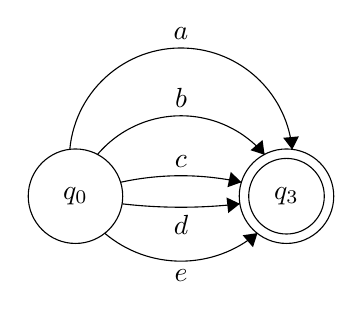
\begin{tikzpicture}[scale=0.2]
		\tikzstyle{every node}+=[inner sep=0pt]
		\draw [black] (26,-28.5) circle (3);
		\draw (26,-28.5) node {$q_3$};
		\draw [black] (26,-28.5) circle (2.4);
		\draw [black] (12.6,-28.5) circle (3);
		\draw (12.6,-28.5) node {$q_0$};
		\draw [black] (15.463,-27.615) arc (102.37767:77.62233:17.901);
		\fill [black] (23.14,-27.61) -- (22.46,-26.96) -- (22.25,-27.93);
		\draw (19.3,-26.7) node [above] {$c$};
		\draw [black] (12.238,-25.544) arc (-185.13671:-354.86329:7.091);
		\fill [black] (26.36,-25.54) -- (26.79,-24.7) -- (25.79,-24.79);
		\draw (19.3,-18.59) node [above] {$a$};
		\draw [black] (13.986,-25.865) arc (139.88963:40.11037:6.949);
		\fill [black] (24.61,-25.87) -- (24.48,-24.93) -- (23.72,-25.58);
		\draw (19.3,-22.89) node [above] {$b$};
		\draw [black] (23.04,-28.984) arc (-83.37239:-96.62761:32.407);
		\fill [black] (23.04,-28.98) -- (22.19,-28.58) -- (22.3,-29.57);
		\draw (19.3,-29.7) node [below] {$d$};
		\draw [black] (24.156,-30.841) arc (-49.67778:-130.32222:7.505);
		\fill [black] (24.16,-30.84) -- (23.22,-30.98) -- (23.87,-31.74);
		\draw (19.3,-33.12) node [below] {$e$};
	\end{tikzpicture}
\end{center}
Interestingly, the regular expression could not be minimised any further. Hence we observe that our procedure does more than a simple syntactic manipulation could achieve.

Glushkov's construction has one more advantage. Because every symbol becomes a state, it's very easy for the user to predict the exact placement of transitions between them. This way, it's easy to embed any property of the transition directly inside the regular expression. For example, suppose that we want to assign come colours to all transitions. Let $B$ stand for blue and $R$ for red. Then it's possible to embed these colours in a expression like follows
\[
aRa(Bb+Rc)R*
\]
which becomes
\[
q_1 R q_2(B q_3+R q_4)R*B
\]
We know that after $q_1$ we can read $q_2$ and along the way we have to cross the color $R$, because it stand in between $q_1$ and $q_2$. Hence it determines that the transition from $q_1$ to $q_2$ should be red. Similarly transition from $q_2$ and $q_3$ must be blue and from $q_2$ and $q_4$ is red. The transition from $q_3$ to $q_3$ will have colour $RB$, because $R$ is under the Kleen closure and $B$ is right before $q_3$. At this point we notice that there must be defined some way of mixing colours. In other words, any meta-information that we wish to embed in our regular expressions must at least form a monoid. The graph resulting from our example looks as follows

\begin{center}
	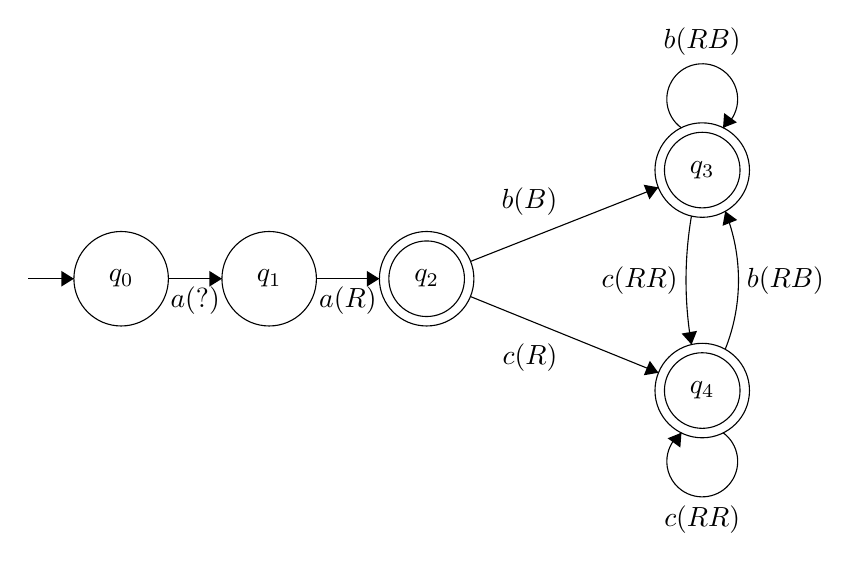
\begin{tikzpicture}[scale=0.2]
		\tikzstyle{every node}+=[inner sep=0pt]
		\draw [black] (12.6,-28.5) circle (3);
		\draw (12.6,-28.5) node {$q_0$};
		\draw [black] (22,-28.5) circle (3);
		\draw (22,-28.5) node {$q_1$};
		\draw [black] (32,-28.5) circle (3);
		\draw (32,-28.5) node {$q_2$};
		\draw [black] (32,-28.5) circle (2.4);
		\draw [black] (49.5,-21.6) circle (3);
		\draw (49.5,-21.6) node {$q_3$};
		\draw [black] (49.5,-21.6) circle (2.4);
		\draw [black] (49.5,-35.6) circle (3);
		\draw (49.5,-35.6) node {$q_4$};
		\draw [black] (49.5,-35.6) circle (2.4);
		\draw [black] (15.6,-28.5) -- (19,-28.5);
		\fill [black] (19,-28.5) -- (18.2,-28) -- (18.2,-29);
		\draw (17.3,-29) node [below] {$a(?)$};
		\draw [black] (25,-28.5) -- (29,-28.5);
		\fill [black] (29,-28.5) -- (28.2,-28) -- (28.2,-29);
		\draw (27,-29) node [below] {$a(R)$};
		\draw [black] (34.79,-27.4) -- (46.71,-22.7);
		\fill [black] (46.71,-22.7) -- (45.78,-22.53) -- (46.15,-23.46);
		\draw (38.53,-24.51) node [above] {$b(B)$};
		\draw [black] (34.78,-29.63) -- (46.72,-34.47);
		\fill [black] (46.72,-34.47) -- (46.17,-33.71) -- (45.79,-34.63);
		\draw (38.57,-32.59) node [below] {$c(R)$};
		\draw [black] (48.815,-32.681) arc (-170.33538:-189.66462:24.31);
		\fill [black] (48.82,-32.68) -- (49.17,-31.81) -- (48.19,-31.98);
		\draw (47.97,-28.6) node [left] {$c(RR)$};
		\draw [black] (50.956,-24.214) arc (21.82527:-21.82527:11.797);
		\fill [black] (50.96,-24.21) -- (50.79,-25.14) -- (51.72,-24.77);
		\draw (52.3,-28.6) node [right] {$b(RB)$};
		\draw [black] (48.177,-18.92) arc (234:-54:2.25);
		\draw (49.5,-14.35) node [above] {$b(RB)$};
		\fill [black] (50.82,-18.92) -- (51.7,-18.57) -- (50.89,-17.98);
		\draw [black] (50.823,-38.28) arc (54:-234:2.25);
		\draw (49.5,-42.85) node [below] {$c(RR)$};
		\fill [black] (48.18,-38.28) -- (47.3,-38.63) -- (48.11,-39.22);
		\draw [black] (6.7,-28.5) -- (9.6,-28.5);
		\fill [black] (9.6,-28.5) -- (8.8,-28) -- (8.8,-29);
	\end{tikzpicture}
\end{center}
Because colours form a monoid, we can use neutral element as a default value for all unspecified edges like $a(?)$. Moreover, it is also possible to attach meta-information to final states. We could imagine that an accepting state is nothing more than a state with a special outgoing transition that goes "outside" of automaton and has no target state. In our example the colours of such "final" transitions are as follows

\begin{center}
	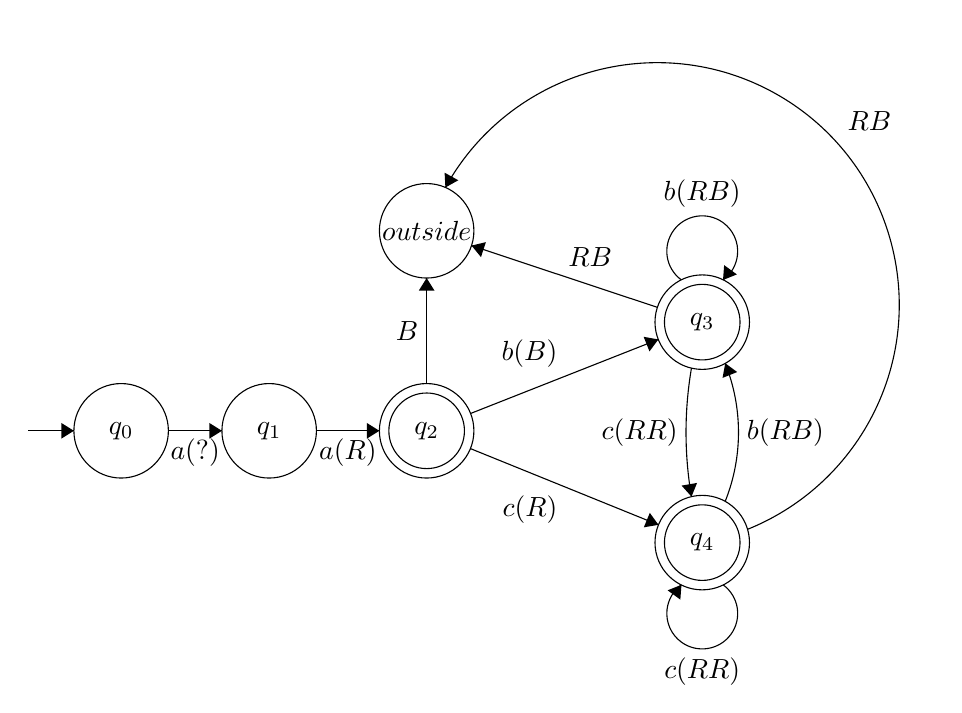
\begin{tikzpicture}[scale=0.2]
		\tikzstyle{every node}+=[inner sep=0pt]
		\draw [black] (12.6,-28.5) circle (3);
		\draw (12.6,-28.5) node {$q_0$};
		\draw [black] (22,-28.5) circle (3);
		\draw (22,-28.5) node {$q_1$};
		\draw [black] (32,-28.5) circle (3);
		\draw (32,-28.5) node {$q_2$};
		\draw [black] (32,-28.5) circle (2.4);
		\draw [black] (49.5,-21.6) circle (3);
		\draw (49.5,-21.6) node {$q_3$};
		\draw [black] (49.5,-21.6) circle (2.4);
		\draw [black] (49.5,-35.6) circle (3);
		\draw (49.5,-35.6) node {$q_4$};
		\draw [black] (49.5,-35.6) circle (2.4);
		\draw [black] (32,-15.8) circle (3);
		\draw (32,-15.8) node {$outside$};
		\draw [black] (15.6,-28.5) -- (19,-28.5);
		\fill [black] (19,-28.5) -- (18.2,-28) -- (18.2,-29);
		\draw (17.3,-29) node [below] {$a(?)$};
		\draw [black] (25,-28.5) -- (29,-28.5);
		\fill [black] (29,-28.5) -- (28.2,-28) -- (28.2,-29);
		\draw (27,-29) node [below] {$a(R)$};
		\draw [black] (34.79,-27.4) -- (46.71,-22.7);
		\fill [black] (46.71,-22.7) -- (45.78,-22.53) -- (46.15,-23.46);
		\draw (38.53,-24.51) node [above] {$b(B)$};
		\draw [black] (34.78,-29.63) -- (46.72,-34.47);
		\fill [black] (46.72,-34.47) -- (46.17,-33.71) -- (45.79,-34.63);
		\draw (38.57,-32.59) node [below] {$c(R)$};
		\draw [black] (48.815,-32.681) arc (-170.33538:-189.66462:24.31);
		\fill [black] (48.82,-32.68) -- (49.17,-31.81) -- (48.19,-31.98);
		\draw (47.97,-28.6) node [left] {$c(RR)$};
		\draw [black] (50.956,-24.214) arc (21.82527:-21.82527:11.797);
		\fill [black] (50.96,-24.21) -- (50.79,-25.14) -- (51.72,-24.77);
		\draw (52.3,-28.6) node [right] {$b(RB)$};
		\draw [black] (48.177,-18.92) arc (234:-54:2.25);
		\draw (49.5,-14.35) node [above] {$b(RB)$};
		\fill [black] (50.82,-18.92) -- (51.7,-18.57) -- (50.89,-17.98);
		\draw [black] (50.823,-38.28) arc (54:-234:2.25);
		\draw (49.5,-42.85) node [below] {$c(RR)$};
		\fill [black] (48.18,-38.28) -- (47.3,-38.63) -- (48.11,-39.22);
		\draw [black] (6.7,-28.5) -- (9.6,-28.5);
		\fill [black] (9.6,-28.5) -- (8.8,-28) -- (8.8,-29);
		\draw [black] (32,-25.5) -- (32,-18.8);
		\fill [black] (32,-18.8) -- (31.5,-19.6) -- (32.5,-19.6);
		\draw (31.5,-22.15) node [left] {$B$};
		\draw [black] (46.65,-20.66) -- (34.85,-16.74);
		\fill [black] (34.85,-16.74) -- (35.45,-17.47) -- (35.76,-16.52);
		\draw (42.38,-18.13) node [above] {$RB$};
		\draw [black] (33.189,-13.051) arc (151.02885:-68.08589:15.372);
		\fill [black] (33.19,-13.05) -- (34.01,-12.59) -- (33.14,-12.11);
		\draw (58.7,-8.86) node [right] {$RB$};
	\end{tikzpicture}
\end{center}
In Solomonoff, the meta-information of interest are transition outputs. We could imagine that strings composed of $R$ and $B$ symbols are the output of transducer.
At this point the reader should appreciate how beautifully and naturally subsequential transducers (automata with output produced at accepting states) are derived from Glushkov's construction. As soon as we enrich regular expressions with meta-information, the state outputs emerge as if they were always there, merely hiding from the view. 

Glushkov's construction together with minimisation procedure and embeded meta-information allowed for efficient implementation of union, concatenation and Kleene closure together with output strings. In order to make the compiler applicable to real-life linguistic problems it also must support context dependent rewrites. This is a heavyweight operations that often constitutes a major performance bottleneck. Our goal was to make it as efficient as possible. 
In order to solve this issue we developed a special lexicographic semiring. This is an innovative solution never seen before.

Suppose we want to replace every occurrence of $abc$ with $d$. Even for such a simple scenario, the corresponding transducer will look rather complex

\begin{center}
	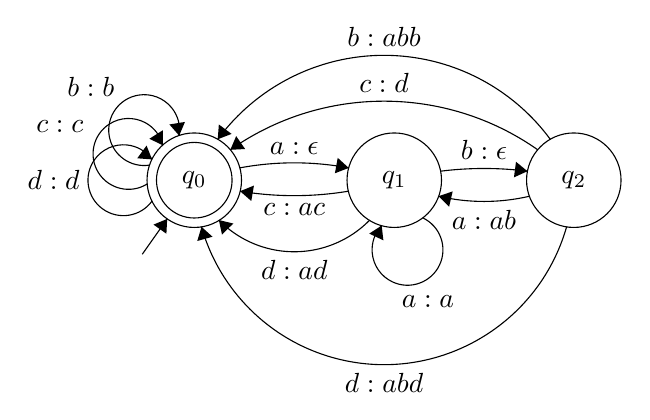
\begin{tikzpicture}[scale=0.2]
		\tikzstyle{every node}+=[inner sep=0pt]
		\draw [black] (12.6,-28.5) circle (3);
		\draw (12.6,-28.5) node {$q_0$};
		\draw [black] (12.6,-28.5) circle (2.4);
		\draw [black] (25.3,-28.5) circle (3);
		\draw (25.3,-28.5) node {$q_1$};
		\draw [black] (36.7,-28.5) circle (3);
		\draw (36.7,-28.5) node {$q_2$};
		\draw [black] (9.3,-33.2) -- (10.88,-30.96);
		\fill [black] (10.88,-30.96) -- (10.01,-31.32) -- (10.83,-31.9);
		\draw [black] (15.493,-27.717) arc (100.57485:79.42515:18.838);
		\fill [black] (22.41,-27.72) -- (21.71,-27.08) -- (21.53,-28.06);
		\draw (18.95,-26.9) node [above] {$a:\epsilon$};
		\draw [black] (28.242,-27.927) arc (97.14298:82.85702:22.176);
		\fill [black] (33.76,-27.93) -- (33.03,-27.33) -- (32.9,-28.32);
		\draw (31,-27.25) node [above] {$b:\epsilon$};
		\draw [black] (14.89,-26.568) arc (125.10167:54.89833:16.974);
		\fill [black] (14.89,-26.57) -- (15.83,-26.52) -- (15.26,-25.7);
		\draw (24.65,-22.98) node [above] {$c:d$};
		\draw [black] (9.77,-27.54) arc (279:-9:2.25);
		\draw (6.03,-23.25) node [above] {$b:b$};
		\fill [black] (11.64,-25.67) -- (12.01,-24.8) -- (11.02,-24.96);
		\draw [black] (9.621,-28.733) arc (302.19859:14.19859:2.25);
		\draw (5.59,-25.11) node [left] {$c:c$};
		\fill [black] (10.6,-26.28) -- (10.6,-25.33) -- (9.75,-25.87);
		\draw [black] (22.385,-29.199) arc (-80.6054:-99.3946:21.044);
		\fill [black] (15.51,-29.2) -- (16.22,-29.82) -- (16.39,-28.84);
		\draw (18.95,-29.98) node [below] {$c:ac$};
		\draw [black] (23.74,-31.033) arc (-44.44662:-135.55338:6.709);
		\fill [black] (14.16,-31.03) -- (14.36,-31.95) -- (15.08,-31.25);
		\draw (18.95,-33.54) node [below] {$d:ad$};
		\draw [black] (14.09,-25.904) arc (143.59719:36.40281:13.12);
		\fill [black] (14.09,-25.9) -- (14.97,-25.56) -- (14.16,-24.96);
		\draw (24.65,-20.07) node [above] {$b:abb$};
		\draw [black] (9.92,-29.823) arc (-36:-324:2.25);
		\draw (5.35,-28.5) node [left] {$d:d$};
		\fill [black] (9.92,-27.18) -- (9.57,-26.3) -- (8.98,-27.11);
		\draw [black] (36.244,-31.457) arc (-15.8876:-164.1124:12.055);
		\fill [black] (13.06,-31.46) -- (12.79,-32.36) -- (13.76,-32.09);
		\draw (24.65,-40.71) node [below] {$d:abd$};
		\draw [black] (33.885,-29.518) arc (-76.88176:-103.11824:12.713);
		\fill [black] (28.11,-29.52) -- (28.78,-30.19) -- (29.01,-29.21);
		\draw (31,-30.35) node [below] {$a:ab$};
		\draw [black] (27.1,-30.885) arc (64.76617:-223.23383:2.25);
		\draw (27.44,-35.78) node [below] {$a:a$};
		\fill [black] (24.5,-31.38) -- (23.71,-31.89) -- (24.61,-32.32);
	\end{tikzpicture}
\end{center}
A much simpler alternative would be the nondeterministic transducer

\begin{center}
	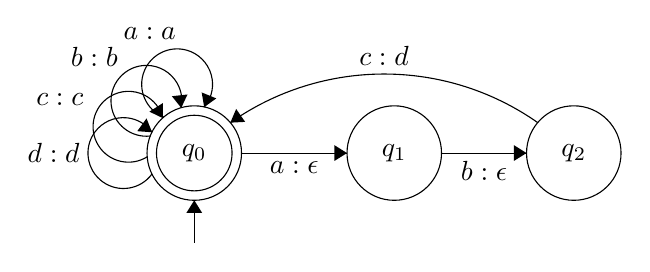
\begin{tikzpicture}[scale=0.2]
		\tikzstyle{every node}+=[inner sep=0pt]
		\draw [black] (12.6,-28.5) circle (3);
		\draw (12.6,-28.5) node {$q_0$};
		\draw [black] (12.6,-28.5) circle (2.4);
		\draw [black] (25.3,-28.5) circle (3);
		\draw (25.3,-28.5) node {$q_1$};
		\draw [black] (36.7,-28.5) circle (3);
		\draw (36.7,-28.5) node {$q_2$};
		\draw [black] (12.6,-34.2) -- (12.6,-31.5);
		\fill [black] (12.6,-31.5) -- (12.1,-32.3) -- (13.1,-32.3);
		\draw [black] (15.6,-28.5) -- (22.3,-28.5);
		\fill [black] (22.3,-28.5) -- (21.5,-28) -- (21.5,-29);
		\draw (18.95,-29) node [below] {$a:\epsilon$};
		\draw [black] (28.3,-28.5) -- (33.7,-28.5);
		\fill [black] (33.7,-28.5) -- (32.9,-28) -- (32.9,-29);
		\draw (31,-29) node [below] {$b:\epsilon$};
		\draw [black] (14.89,-26.568) arc (125.10167:54.89833:16.974);
		\fill [black] (14.89,-26.57) -- (15.83,-26.52) -- (15.26,-25.7);
		\draw (24.65,-22.98) node [above] {$c:d$};
		\draw [black] (9.815,-27.417) arc (276.48816:-11.51184:2.25);
		\draw (6.25,-23.04) node [above] {$b:b$};
		\fill [black] (11.77,-25.63) -- (12.17,-24.78) -- (11.18,-24.89);
		\draw [black] (9.621,-28.733) arc (302.19859:14.19859:2.25);
		\draw (5.59,-25.11) node [left] {$c:c$};
		\fill [black] (10.6,-26.28) -- (10.6,-25.33) -- (9.75,-25.87);
		\draw [black] (9.92,-29.823) arc (-36:-324:2.25);
		\draw (5.35,-28.5) node [left] {$d:d$};
		\fill [black] (9.92,-27.18) -- (9.57,-26.3) -- (8.98,-27.11);
		\draw [black] (10.668,-26.22) arc (248.00665:-39.99335:2.25);
		\draw (9.77,-21.33) node [above] {$a:a$};
		\fill [black] (13.23,-25.58) -- (14,-25.03) -- (13.07,-24.65);
	\end{tikzpicture}
\end{center}
The problem with such solution is that for input strings like $aabcb$ both outputs $aabcb$ and $adb$ are generated. If only there was a way to assign priority to some outputs in order to disambiguate them, then context dependent rewrites could be expressed by much simpler automata. This is precisely what lexicographic weights are for. 

Consider the following fragment of automaton and suppose that it's possible to simultaneously nondeterministically reach both $q_2$ and $q_1$.
\begin{center}
	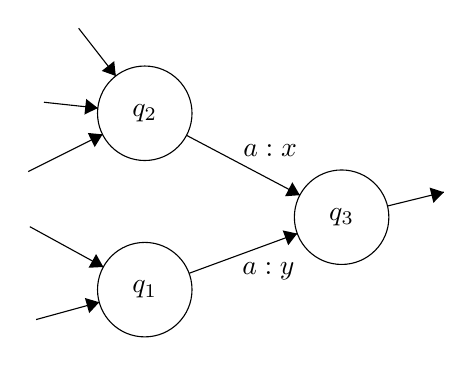
\begin{tikzpicture}[scale=0.2]
		\tikzstyle{every node}+=[inner sep=0pt]
		\draw [black] (24.2,-33.1) circle (3);
		\draw (24.2,-33.1) node {$q_1$};
		\draw [black] (36.7,-28.5) circle (3);
		\draw (36.7,-28.5) node {$q_3$};
		\draw [black] (24.2,-21.9) circle (3);
		\draw (24.2,-21.9) node {$q_2$};
		\draw [black] (27.02,-32.06) -- (33.88,-29.54);
		\fill [black] (33.88,-29.54) -- (32.96,-29.34) -- (33.31,-30.28);
		\draw (32.05,-31.34) node [below] {$a:y$};
		\draw [black] (26.85,-23.3) -- (34.05,-27.1);
		\fill [black] (34.05,-27.1) -- (33.57,-26.28) -- (33.11,-27.17);
		\draw (32.16,-24.69) node [above] {$a:x$};
		\draw [black] (16.8,-25.6) -- (21.52,-23.24);
		\fill [black] (21.52,-23.24) -- (20.58,-23.15) -- (21.02,-24.05);
		\draw [black] (16.9,-29.1) -- (21.57,-31.66);
		\fill [black] (21.57,-31.66) -- (21.11,-30.84) -- (20.63,-31.71);
		\draw [black] (17.3,-35) -- (21.31,-33.9);
		\fill [black] (21.31,-33.9) -- (20.4,-33.63) -- (20.67,-34.59);
		\draw [black] (17.8,-21.2) -- (21.22,-21.57);
		\fill [black] (21.22,-21.57) -- (20.48,-20.99) -- (20.37,-21.98);
		\draw [black] (20,-16.5) -- (22.36,-19.53);
		\fill [black] (22.36,-19.53) -- (22.26,-18.59) -- (21.47,-19.21);
		\draw [black] (39.61,-27.79) -- (43.19,-26.91);
		\fill [black] (43.19,-26.91) -- (42.29,-26.62) -- (42.53,-27.59);
	\end{tikzpicture}
\end{center}
If the next input symbol is $a$, then the transducer will reach state $q_3$ and generate two outputs - one ending in $x$ and the other in $y$. If the automaton later accepts it will produce at least two ambiguous outputs.
Lexicographic weights allow us to assign priority to different transitions.
In the following example, only the output ending in $x$ will reach state $q_3$ and the other ending in $y$ will be discarded because it came to $q_3$ over transition with lower weight.
\begin{center}
	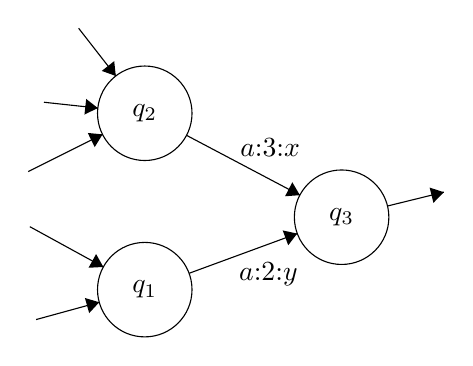
\begin{tikzpicture}[scale=0.2]
		\tikzstyle{every node}+=[inner sep=0pt]
		\draw [black] (24.2,-33.1) circle (3);
		\draw (24.2,-33.1) node {$q_1$};
		\draw [black] (36.7,-28.5) circle (3);
		\draw (36.7,-28.5) node {$q_3$};
		\draw [black] (24.2,-21.9) circle (3);
		\draw (24.2,-21.9) node {$q_2$};
		\draw [black] (27.02,-32.06) -- (33.88,-29.54);
		\fill [black] (33.88,-29.54) -- (32.96,-29.34) -- (33.31,-30.28);
		\draw (32.05,-31.34) node [below] {$a{:}2{:}y$};
		\draw [black] (26.85,-23.3) -- (34.05,-27.1);
		\fill [black] (34.05,-27.1) -- (33.57,-26.28) -- (33.11,-27.17);
		\draw (32.16,-24.69) node [above] {$a{:}3{:}x$};
		\draw [black] (16.8,-25.6) -- (21.52,-23.24);
		\fill [black] (21.52,-23.24) -- (20.58,-23.15) -- (21.02,-24.05);
		\draw [black] (16.9,-29.1) -- (21.57,-31.66);
		\fill [black] (21.57,-31.66) -- (21.11,-30.84) -- (20.63,-31.71);
		\draw [black] (17.3,-35) -- (21.31,-33.9);
		\fill [black] (21.31,-33.9) -- (20.4,-33.63) -- (20.67,-34.59);
		\draw [black] (17.8,-21.2) -- (21.22,-21.57);
		\fill [black] (21.22,-21.57) -- (20.48,-20.99) -- (20.37,-21.98);
		\draw [black] (20,-16.5) -- (22.36,-19.53);
		\fill [black] (22.36,-19.53) -- (22.26,-18.59) -- (21.47,-19.21);
		\draw [black] (39.61,-27.79) -- (43.19,-26.91);
		\fill [black] (43.19,-26.91) -- (42.29,-26.62) -- (42.53,-27.59);
	\end{tikzpicture}
\end{center}
Lexicographic weights allow to make the transducers even more compact. We proved that there exist weighted automata exponentially smaller than even the smallest unweighted nondeterministic ones. In the presence of lexicographic weights, context-dependent rewrites become expressible directly in Glushkov's construction, without the need for calling any "external operations". 

In the tasks of natural language processing it's common to work with large alphabets. User input might contain unexpected sequences like math symbols, foreign words or even emojis and other UNICODE entities. The regular expressions should handle such cases gracefully, especially when using wildcards such as \texttt{.*} or \texttt{\textbackslash p\{Lu\}}. Representation of large character classes is a challenging task for finite state automata. In order to use the dot wildcard in UNICODE, the automaton would require millions of transitions, one for each individual symbol. 
In order to optimise this, Solomonoff employs symbolic transitions. While classic automata have edges labelled with individual symbols, our transducers have edges that span entire ranges. A range is easy to encode in computers memory. It's enough to store the first and last symbol. Below is an example of classical finite state automaton

\begin{center}
	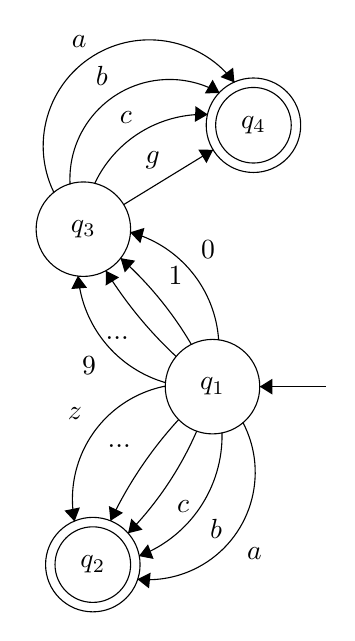
\begin{tikzpicture}[scale=0.2]
		\tikzstyle{every node}+=[inner sep=0pt]
		\draw [black] (21.9,-33.8) circle (3);
		\draw (21.9,-33.8) node {$q_1$};
		\draw [black] (14.3,-45.1) circle (3);
		\draw (14.3,-45.1) node {$q_2$};
		\draw [black] (14.3,-45.1) circle (2.4);
		\draw [black] (13.7,-23.8) circle (3);
		\draw (13.7,-23.8) node {$q_3$};
		\draw [black] (24.5,-17.2) circle (3);
		\draw (24.5,-17.2) node {$q_4$};
		\draw [black] (24.5,-17.2) circle (2.4);
		\draw [black] (29.1,-33.8) -- (24.9,-33.8);
		\fill [black] (24.9,-33.8) -- (25.7,-34.3) -- (25.7,-33.3);
		\draw [black] (23.827,-36.068) arc (27.74974:-95.59664:6.819);
		\fill [black] (17.13,-46.03) -- (17.87,-46.61) -- (17.97,-45.61);
		\draw (24.06,-44.39) node [right] {$a$};
		\draw [black] (22.505,-36.721) arc (1.21842:-69.06533:8.204);
		\fill [black] (17.23,-44.56) -- (18.16,-44.74) -- (17.8,-43.81);
		\draw (21.72,-42.81) node [right] {$b$};
		\draw [black] (20.897,-36.625) arc (-23.51659:-44.33031:21.62);
		\fill [black] (16.54,-43.11) -- (17.46,-42.88) -- (16.74,-42.18);
		\draw (19.62,-41.4) node [right] {$c$};
		\draw [black] (15.425,-42.321) arc (154.65938:137.49372:25.965);
		\fill [black] (15.42,-42.32) -- (16.22,-41.81) -- (15.32,-41.38);
		\draw (16.74,-37.6) node [left] {$...$};
		\draw [black] (13.142,-42.355) arc (-168.87:-258.9769:7.316);
		\fill [black] (13.14,-42.36) -- (13.48,-41.47) -- (12.5,-41.67);
		\draw (13.64,-35.52) node [left] {$z$};
		\draw [black] (16.674,-23.995) arc (74.9508:3.75271:7.609);
		\fill [black] (16.67,-24) -- (17.32,-24.69) -- (17.58,-23.72);
		\draw (21.14,-25.09) node [right] {$0$};
		\draw [black] (16.065,-25.642) arc (48.30476:30.39874:22.759);
		\fill [black] (16.06,-25.64) -- (16.33,-26.55) -- (16.99,-25.8);
		\draw (19.08,-26.77) node [right] {$1$};
		\draw [black] (19.593,-31.885) arc (-132.96338:-148.33311:26.34);
		\fill [black] (15.13,-26.44) -- (15.12,-27.38) -- (15.97,-26.86);
		\draw (16.62,-30.74) node [left] {$...$};
		\draw [black] (18.929,-33.549) arc (-105.96776:-175.32874:7.713);
		\fill [black] (13.36,-26.76) -- (12.93,-27.6) -- (13.93,-27.52);
		\draw (14.53,-32.46) node [left] {$9$};
		\draw [black] (11.835,-21.482) arc (-153.92109:-323.21978:6.741);
		\fill [black] (23.29,-14.48) -- (23.21,-13.54) -- (22.41,-14.14);
		\draw (13.43,-12.27) node [above] {$a$};
		\draw [black] (12.853,-20.951) arc (-177.02573:-300.11514:6.33);
		\fill [black] (22.35,-15.15) -- (21.91,-14.31) -- (21.41,-15.18);
		\draw (14.87,-14.72) node [above] {$b$};
		\draw [black] (14.415,-20.906) arc (154.87614:87.98299:7.638);
		\fill [black] (21.6,-16.52) -- (20.82,-15.99) -- (20.78,-16.99);
		\draw (16.4,-17.13) node [above] {$c$};
		\draw [black] (16.26,-22.24) -- (21.94,-18.76);
		\fill [black] (21.94,-18.76) -- (21,-18.75) -- (21.52,-19.61);
		\draw (18.1,-20) node [above] {$g$};
	\end{tikzpicture}
\end{center}
and an equivalent symbolic automaton that uses closed ranges of symbols as transition predicates
\begin{center}
	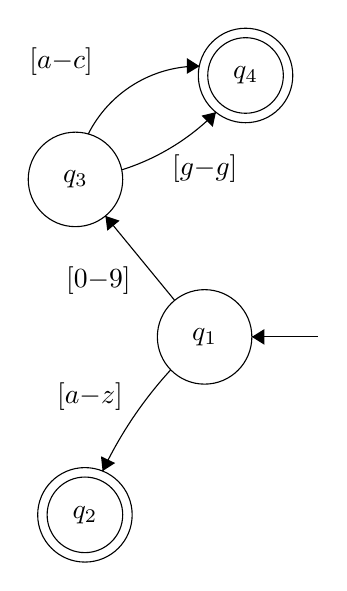
\begin{tikzpicture}[scale=0.2]
		\tikzstyle{every node}+=[inner sep=0pt]
		\draw [black] (21.9,-33.8) circle (3);
		\draw (21.9,-33.8) node {$q_1$};
		\draw [black] (14.3,-45.1) circle (3);
		\draw (14.3,-45.1) node {$q_2$};
		\draw [black] (14.3,-45.1) circle (2.4);
		\draw [black] (13.7,-23.8) circle (3);
		\draw (13.7,-23.8) node {$q_3$};
		\draw [black] (24.5,-17.2) circle (3);
		\draw (24.5,-17.2) node {$q_4$};
		\draw [black] (24.5,-17.2) circle (2.4);
		\draw [black] (29.1,-33.8) -- (24.9,-33.8);
		\fill [black] (24.9,-33.8) -- (25.7,-34.3) -- (25.7,-33.3);
		\draw [black] (15.425,-42.321) arc (154.65938:137.49372:25.965);
		\fill [black] (15.42,-42.32) -- (16.22,-41.81) -- (15.32,-41.38);
		\draw (16.74,-37.6) node [left] {$[a {-} z]$};
		\draw [black] (20,-31.48) -- (15.6,-26.12);
		\fill [black] (15.6,-26.12) -- (15.72,-27.06) -- (16.5,-26.42);
		\draw (17.24,-30.23) node [left] {$[0{-}9]$};
		\draw [black] (14.506,-20.929) arc (153.34454:89.5146:7.838);
		\fill [black] (21.58,-16.61) -- (20.78,-16.1) -- (20.77,-17.1);
		\draw (12.79,-17.25) node [above] {$[a{-}c]$};
		\draw [black] (22.625,-19.535) arc (-44.65667:-72.4842:14.6);
		\fill [black] (22.62,-19.53) -- (21.71,-19.75) -- (22.42,-20.46);
		\draw (21.91,-22.23) node [below] {$[g{-}g]$};
	\end{tikzpicture}
\end{center}
Compilation of transducers is the core part of our library but in order to make the automata useful there must be a way to execute them. Deterministic transducers and Mealy machines could be evaluated in linear time. Nondeterministic automata are more expensive. The computation might branch and automaton could be in multiple states simultaneously. Using dynamic programming it's possible to build a table with rows representing consecutive symbols of input string and each column keeping track of one state. 
At each step of execution, one input symbol is read and one row in the table is filled based on the contents of previous row. Below is an example of nondeterministic finite state automaton and its corresponding evaluation table after reading input string $aba$.

\begin{center}
	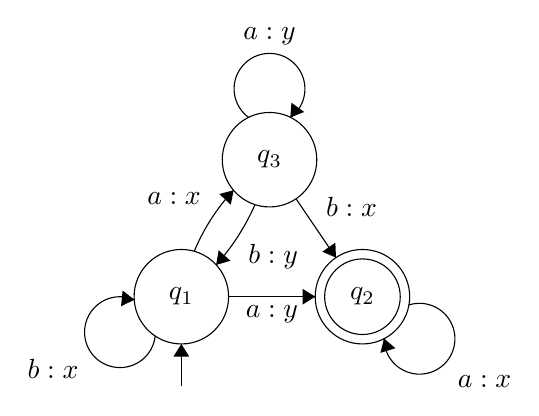
\begin{tikzpicture}[scale=0.2]
		\tikzstyle{every node}+=[inner sep=0pt]
		\draw [black] (16.5,-23.2) circle (3);
		\draw (16.5,-23.2) node {$q_1$};
		\draw [black] (28,-23.2) circle (3);
		\draw (28,-23.2) node {$q_2$};
		\draw [black] (28,-23.2) circle (2.4);
		\draw [black] (22.1,-14.5) circle (3);
		\draw (22.1,-14.5) node {$q_3$};
		\draw [black] (19.5,-23.2) -- (25,-23.2);
		\fill [black] (25,-23.2) -- (24.2,-22.7) -- (24.2,-23.7);
		\draw (22.25,-23.7) node [below] {$a:y$};
		\draw [black] (17.318,-20.321) arc (157.50332:136.95968:12.951);
		\fill [black] (19.82,-16.44) -- (18.91,-16.68) -- (19.64,-17.36);
		\draw (17.77,-16.95) node [left] {$a:x$};
		\draw [black] (23.78,-16.98) -- (26.32,-20.72);
		\fill [black] (26.32,-20.72) -- (26.28,-19.77) -- (25.45,-20.34);
		\draw (25.66,-17.5) node [right] {$b:x$};
		\draw [black] (21.18,-17.35) arc (-23.77693:-41.76007:14.582);
		\fill [black] (18.71,-21.18) -- (19.62,-20.92) -- (18.87,-20.25);
		\draw (20.72,-20.68) node [right] {$b:y$};
		\draw [black] (20.777,-11.82) arc (234:-54:2.25);
		\draw (22.1,-7.25) node [above] {$a:y$};
		\fill [black] (23.42,-11.82) -- (24.3,-11.47) -- (23.49,-10.88);
		\draw [black] (30.942,-23.725) arc (107.61565:-180.38435:2.25);
		\draw (34.02,-28.59) node [right] {$a:x$};
		\fill [black] (29.37,-25.85) -- (29.14,-26.77) -- (30.09,-26.47);
		\draw [black] (14.841,-25.685) arc (-5.99178:-293.99178:2.25);
		\draw (10,-27.81) node [left] {$b:x$};
		\fill [black] (13.52,-23.39) -- (12.77,-22.81) -- (12.67,-23.81);
		\draw [black] (16.5,-28.9) -- (16.5,-26.2);
		\fill [black] (16.5,-26.2) -- (16,-27) -- (17,-27);
	\end{tikzpicture}
\end{center}

\begin{table}[!htbp]
	\centering
	\begin{tabular}{|l|l|l|l|}
		\hline
		symbol                                                          & $q_1$ & $q_2$ & $q_3$ \\ \hline
		\begin{tabular}[c]{@{}l@{}}initial\\ configuration\end{tabular} & 1    & 0    & 0    \\ \hline
		a                                                               & 0    & 1    & 1    \\ \hline
		b                                                               & 1    & 1    & 0    \\ \hline
		a                                                               & 0    & 1    & 1    \\ \hline
	\end{tabular}
\end{table}

By the end of evaluating such a table, it's enough to scan the last row to find a column of some accepting state. In the above example, such a state is $q_2$ and we can observe that it's active in the last row.

In case of transducers, we not only want to know, whether the string was accepted or not but also the output generated along the way. In order to do this  the table can be backtracked from the accepting state backwards. For the backtracking step to be possible, we need to store information about source state of each taken transition. 

\begin{table}[!htbp]
	\centering
	\begin{tabular}{|l|l|l|l|}
		\hline
		symbol                                                          & $q_1$ & $q_2$ & $q_3$ \\ \hline
		\begin{tabular}[c]{@{}l@{}}initial\\ configuration\end{tabular} & $q_1$    & $\emptyset$    & $\emptyset$    \\ \hline
		a                                                               & $\emptyset$    & $q_1$    & $q_1$    \\ \hline
		b                                                               & $q_3$    & $q_3$    & $\emptyset$    \\ \hline
		a                                                               & $\emptyset$    & $q_1$    & $q_1$    \\ \hline
	\end{tabular}
\end{table}
Assuming that every transition is uniquely determined by its symbol, source state and target state (in other words $\delta:Q\times \Sigma\times Q \rightarrow \Gamma^*$), it becomes possible to use such evaluation table to find the exact accepting path in automaton and collect all the outputs printed along the way. 

This algorithm has been made even more efficient by using techniques from graph theory. Every automaton is a directed graph that could be represented as adjacency matrix. An example is shown below.
\begin{table}[!htbp]
	\centering
	\begin{tabular}{|l|l|l|l|}
		\hline
		adjacency & $q_1$      & $q_2$ & $q_3$      \\ \hline
		$q_1$     & b:x        & a:y   & a:x        \\ \hline
		$q_2$     & $\emptyset$ & a:x   & $\emptyset$ \\ \hline
		$q_3$     & b:y        & b:x   & a:y        \\ \hline
	\end{tabular}
\end{table}

Sparse graphs can be optimised and instead of using matrix it's possible to only store the list of adjacent vertices. 
\[
(q_1,b:x,q_1), (q_1,a:y,q_2), (q_1,a:x,q_3), (q_2,a:x,q_2), (q_3,b:y,q_3), ...
\]
Nondeterministic  automata very often are the perfect example of sparse graphs. Hence instead of using evaluation table, it's better to use a list of states nondeterministically reached at any given step of evaluation. 
\begin{table}[!htbp]
	\centering
	\begin{tabular}{|l|l|}
		\hline
		symbol                                                          & list \\ \hline
		\begin{tabular}[c]{@{}l@{}}initial\\ configuration\end{tabular} & $q_1$ \\ \hline
		a                                                               & $q_2,q_3$    \\ \hline
		b                                                               & $q_1,q_2$    \\ \hline
		a                                                               & $q_2,q_3$    \\ \hline
	\end{tabular}
\end{table}

The backtracking can be made efficient by storing pointer to source state of any taken transition.

\begin{table}[!htbp]
	\centering
	\begin{tabular}{|l|l|}
		\hline
		symbol                                                          & list \\ \hline
		\begin{tabular}[c]{@{}l@{}}initial\\ configuration\end{tabular} & $q_1(\mbox{ from }q_1)$ \\ \hline
		a                                                               & $q_2(\mbox{ from }q_1), q_3(\mbox{ from }q_1)$    \\ \hline
		b                                                               & $ q_1(\mbox{ from }q_3), q_2(\mbox{ from }q_3)$    \\ \hline
		a                                                               & $q_2(\mbox{ from }q_1),  q_3(\mbox{ from }q_1)$    \\ \hline
	\end{tabular}
\end{table}

Glushkov's construction relies on building three sets: the set of initial symbols, final symbols and 2-factor strings (that is, all substrings of length 2). The early prototype versions of Solomonoff would represent sets as bitsets, where each bit specifies whether element belongs to the set or not. This representation simplified implementation of many algorithms but was highly inefficient. Later implementation used hash sets instead. While hash maps have constant insertions and deletions, they ensure it at the cost of larger memory consumption. During benchmarks on real-life datasets, Solomonoff would often run out of memory and crash.  The final version uses signly linkged graphs backed by arrays. This provides the highest efficiency with smallest memory footprint but it non-trivial to implement. The optimisation relies on representing sparse sets as arrays of elements. This approach proved to be the best choice, because Glushkov's construction inherently ensures uniqueness of all inserted elements (hence using hashes to search for duplicates before insertion was not necessary)  and it does not use deletions. As a result any array was guaranteed to behave like a set.

The standard definition of Glushkov's construction produces set of 2-factors as its output. Then a separate procedure would be necessary to collect all such strings and convert them into a graph of automaton. We found a way to make it more efficient and build the graph directly. The step of building 2-factors was entirely bypassed. This provided even further optimisation.

One of the core features of Solomonoff is the algorithm for detecting ambiguous nondeterminism. Advance-and-delay procedure can check functionality of automaton in quadratic time. While the compiler does provide implementation of this procedure, it is not used for checking functionality. Instead we use a simpler algorithm for checking strong functionality of lexicographic weights. While the performance difference between the two is negligable, the advantage of our approach comes from  better error messages in case of nondeterminism. If some lexicographic weights are in conflict with each other, compiler can point user to the exact line and column of text where the conflict arises, whereas advance-and-delay might miss the origin of problem and only fail further down the line.



\bibliographystyle{BibTeXtran}   % (uses file "BibTeXtran.bst")
\bibliography{BibTeXrefs}    







\end{document}
